\section{Networks and complex systems}
\label{sec:networks}

Networks are often used to represent complex systems composed of many parts, such as individual people, animals, or atoms. Their study focuses on the nature and structure of interactions between these components. Just as a universe of only non-interacting particles would be a lifeless soup, a collection of people who never interact is boring and unrealistic to study. The network of interactions between the many pieces makes the system “complex.” 

\subsection{Representing network data}

In a network (or "graph") these components are abstractly represented as \emph{nodes} ("vertices") and the interactions are represented as \emph{edges}, lines that connect interacting nodes with each other. This simple framework is flexible enough to span a rich variety of applications and data under various interpretations of the nodes and edges.

\begin{figure}
    \centering
    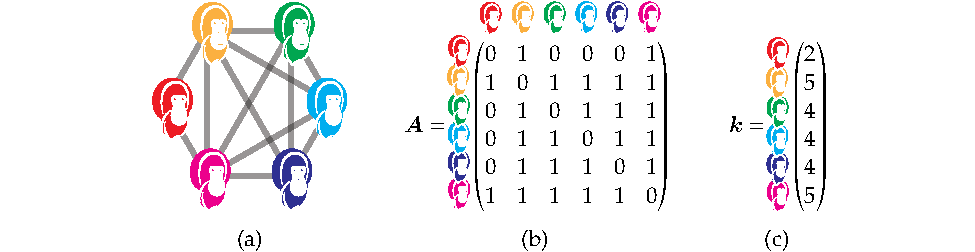
\includegraphics{max_dissertation//chapters//figures//chp1/orangutan-network.pdf}
    \caption{Network of interactions observed by Setia~\etal~\cite{SV07} among $n = 6$ orangutans represented (a) as a graph and (b) as an adjacency matrix~$\mat{A}$. (c) The node degrees~$\vec{k}$, the number of interactions of each orangutan.}
    \label{fig:orangutan-network}
\end{figure}

An example network is given in Figure~\ref{fig:orangutan-network}a. There the colored nodes represent 6 Indonesian flanged male orangutans who are connected by an edge if a vocalization between them was observed in a study by Setia~\etal~\cite{SV07}. As reflected in the graph, 5 of the 6 orangutans form a \emph{clique} of nodes that each interact with each other while the remaining ape represented in red interfaced with only the orange and magenta orangutans. 

Such a network on~$n$ nodes is often alternatively represented by a $n \times n$ \emph{adjacency matrix}~$\mat{A}$, whose entry~$A_{ij}$ for~$i,j = 1,...,n$ is equal to $1$ if nodes~$i$ and~$j$ interact and~$0$ otherwise. Figure~\ref{fig:orangutan-network}b shows the orangutan network in this format with the rows and columns labeled by the orangutan they reference. This matrix and its properties naturally convey information about the network. For example the vector~$\vec{k}$ of row (or column) sums of the adjacency matrix \begin{align}
    k_i = \sum_{j=1}^n A_{ij}, \qquad i = 1,...,n,
\end{align}
gives the \emph{degree} of each node, the total number of edges connected to it.

These degrees of our apes are given in Figure~\ref{fig:orangutan-network}c. The red orangutan is the only node with degree 2, while the orange and magenta orangutans have degree 5 as they both connect to every other orangutan. This simple measure of counting connections captures a sense of \emph{centrality} within the network as certain orangutans appear more disposed to interact than others. This sort of variation in the degrees is typical of real networks, particularly within large data sets. We further discuss how the distribution of the degrees can be modeled and interpreted in Section~\ref{sec:configuration-model}.

The edges in Figure~\ref{fig:orangutan-network} are bidirectional since they symmetrically represent whether any interaction occurred between a pair of orangutans. The network is therefore an \emph{undirected} graph and has a symmetric adjacency matrix. Although such undirected graphs are very common, and the focus of much of this thesis, many systems possess asymmetric interactions. In fact, in their observations Setia~\etal~not only recorded whether a pair interacted but also which orangutan was dominant over the other from their pattern of vocalizations. We can add this layer of information to the network by converting it to a \emph{directed} graph, where each edge is now represented by an arrow that points from the dominant "winner" of the interaction to the submissive "loser." 

The original network of Fig.~\ref{fig:orangutan-network} is also a \emph{simple} graph as interactions are binary -- two nodes either do or do not connect and no node connects to itself. However some pairs of orangutans interacted more than once over the course of the study, a feature we can represent with a \emph{multigraph} where nodes can connect with more than one edge and \emph{self-edges} can connect a node to itself. Although self-edges are not present in the orangutan context, such self-interactions arise in other settings. In a food web of predation among species, for example, cannibalism within a species is represented with a self-edge. 

By incorporating these generalizations, the network of Figure~\ref{fig:orangutan-multigraph}a represents the full detail of the data set of Setia~\etal~\cite{SV07}. Where the original network of Figure~\ref{fig:orangutan-network} represents \emph{if} a pair of orangutans interact, this new network gives fuller context as to the \emph{nature} of the interactions. The adjacency matrix in Figure~\ref{fig:orangutan-multigraph}b is no longer a symmetric binary matrix as~$A_{ij}$ now represents the number of directed edges from node~$i$ to node~$j$. This asymmetry generates two distinct notions of degree. Figure~\ref{fig:orangutan-multigraph}c contains the row sums of the matrix, the \emph{out-degrees}~$\vec{k}^{\text{out}}$, that indicate the number of edges pointing away from a given node, in this case the number of times each orangutan had a dominant interaction. In Figure~\ref{fig:orangutan-multigraph}d the column sums of the matrix give the \emph{in-degrees}~$\vec{k}^{\text{in}}$, the count of edges pointing towards each node, the number of times each orangutan had a submissive interaction. The directions of the data and resulting degrees give further insight to the social world of the orangutans. For example the magenta orangutan has~$k_i^{\text{out}} = 9, k_i^{\text{in}} = 0$ and so was dominant in each of his 9 interactions, suggesting that he holds a prime position in the orangutans' social hierarchy. 

\begin{figure}
    \centering
    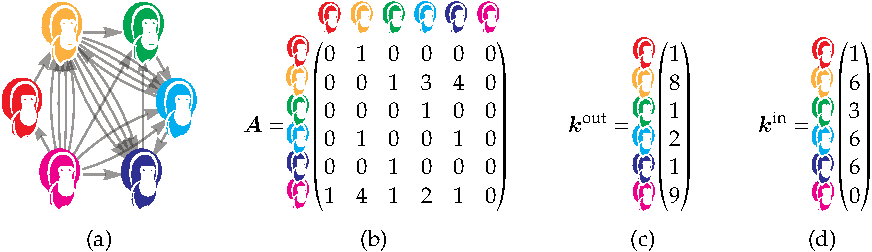
\includegraphics{max_dissertation//chapters//figures//chp1/orangutan-multigraph.pdf}
    \caption{Directed multigraph of dominance interactions observed among $n = 6$ orangutans~\cite{SV07} represented (a) as a graph and (b) as an adjacency matrix~$\mat{A}$. (c) The out-degrees~$\vec{k}^{\text{out}}$ and (d) the in-degrees~$\vec{k}^{\text{in}}$ are also given, respectively counting the number of times each orangutan exhibits a dominant or submissive interaction.}
    \label{fig:orangutan-multigraph}
\end{figure}

Further adornments of networks are often made to represent further detail. In a trade network each edge could carry a continuous weight that reports trade volume between two countries, an example of a \emph{weighted graph} represented by a continuous adjacency matrix~\cite{DNAL15}. Edges can also be differentiated by their type, for example friendships in a social network may be associated to different contexts like work, hobbies, or social media forming a \emph{multilayer} network of connections between people~\cite{CGZ13, Kivela14}. 

Higher-order interactions between triplets and larger groups of nodes may be also be represented either as hypergraphs or bipartite networks, although they are beyond our present scope. In this thesis we focus on interactions between only pairs of nodes, so-called \emph{dyadic interactions}. In fact most of this thesis focuses only on the nature of the simple, undirected networks exemplified by Figure~\ref{fig:orangutan-network}. Only in Section~\ref{chp:hierarchies} do we consider directions of edges and the patterns they reveal. 

Although adding increasingly descriptive context and metadata to networks helps to paint a fuller picture of any particular application, by stripping systems down to a simple pattern of interactions it is possible to treat them within a unified language of network science and understand similarities and differences between them. In this thesis we focus on two common structures found in networks across contexts, group and hierarchical structure. 

\subsection{Group structure}
\label{sec:group-structure}
The nodes that make up a network often possess distinct group identities. Animals are distinguished by species, atoms differ by atomic number, and students belong to various clubs and social groups. These group labels may then influence the interactions among the nodes as, for example, students are often friends with others in the same school club. Figure~\ref{fig:community-examples} gives four examples of real networks where the color of each node indicates which group it belongs to. In each system these group affiliations guide the pattern of connections as nodes of the same group share the same structural role.

\begin{figure}
    \centering
    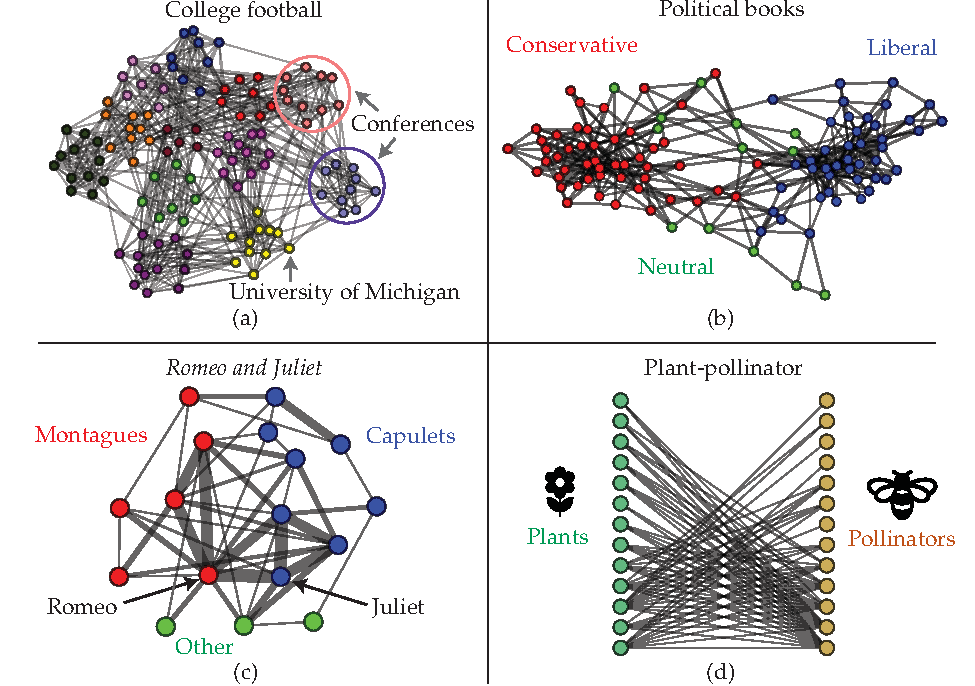
\includegraphics{max_dissertation//chapters//figures//chp1/community-examples.pdf}
    \caption{Four examples of community structure in networks. (a) American football matches among Division IA colleges in the 2000 regular season~\cite{GN02}. Most matches occur within the labeled "conferences" that the teams belong to. (b) Network of political books frequently copurchased on Amazon.com near the 2004 U.S. presidential election labeled by political lean. (c) Network of characters in Shakespeare's \textit{Romeo and Juliet} where edge thickness indicates frequency of interaction. The house each character belongs to in the work, Montague or Capulet, is highlighted. (d) Bipartite network of plant-pollinator interactions~\cite{BMM09}}.
    \label{fig:community-examples}
\end{figure}

Figure~\ref{fig:community-examples}a contains a network of~$616$ American football matches played among~$115$ Division IA colleges in the 2000 regular season~\cite{GN02}. Each year these football teams group into conferences that agree to play a certain number of matches, often 8, against other teams in the same conference. While matches out-of-conference are permitted, they occur more rarely as they are organized on an ad hoc basis from year to year. The conference system thus gives teams an \emph{assortative} preference to play teams of the same group. Over the course of the season the network of matches then carries a clear signature of the conferences that inform them.

Similarly assortative structure is found in Figure~\ref{fig:community-examples}b, a network of~$105$ political books frequently copurchased on Amazon.com near the 2004 U.S. presidential election. Here the books are colored by the political lean of their content, characterized by V. Krebs in unpublished work. Books of the same political bent are typically purchased together, either both liberal or both conservative. Rarely does someone order both a conservative and liberal book in the data set. In this case the observed assortative structure is not imposed by a collective agreement like the football conference system but rather emerges from individual decisions as an effect of systemic political polarization. 

In networks of social ties, people and animals often organize into tightly knit \emph{communities} that prefer to interact amongst themselves. Figure~\ref{fig:community-examples}c contains a (fictional) example of such a network among characters in Shakespeare's \textit{Romeo and Juliet}. Character interactions, defined as subsequent appearances in the same scene, form the edges of this multigraph, where the edge thickness reflects the frequency of the interaction. In the play most characters belong to one of two groups, either Romeo's House of Montague or Juliet's House of Capulet. Interactions between characters are indeed mostly contained within each house. The narrative, however, revolves around the titular exception to this pattern. Later in this thesis we will observe similar patterns of communities across social networks and quantify the extent to which their group boundaries are crossed.

Not all group structures are assortative in this manner. In fact many network data sets are~\emph{bipartite}, meaning they consist of two groups of nodes that never interact within their own group, only with the opposite group: a fully \emph{disassortative} structure. Figure~\ref{fig:community-examples}d gives an example of a bipartite plant-pollinator network. In it 13 species of Brazilian oil-flowers are connected to which of 13 species of pollinators visited them over the course of a study by Berezza~\etal~\cite{BMM09}. In this setting the nodes are naturally sorted by their role as either a plant or a pollinator. Being a bipartite network, all interactions occur only between a plant and a pollinator, never directly between two plants or two pollinators. 

In these examples and beyond networks possess a variety of group structures, distinguished both in the number of groups present and how those groups inform the pattern of interactions. In the four examples of Figure~\ref{fig:community-examples}, group identities can be gleaned from context outside the network of interactions. However in many contexts only the pattern of connections is known, although nodes may still meaningfully belong to groups that influence that structure. 

In this setting a key task of network science is \emph{community detection}, to analyze a network and identify if group structure exists, identify the groups, and characterize their structural relationships. A variety of approaches have been developed for this task, including novel methods discussed in Section~\ref{chp:group-structure} of this thesis. The groups inferred from the network can then be interpreted in their own right or compared to known group labels. In Section~\ref{chp:information} we will discuss and refine how the difference between these inferred and true groups can be quantified.

\subsection{Hierarchy structure}
\label{sec:hierarchy-structure}
As in our orangutan example, network interactions are often directed. Edges in a directed graph variously run from a source to a target, a winner to a loser, a leader to a follower. Across a system these asymmetries often follow a coherent direction within a hierarchy of the nodes. In a sports context this may be a hierarchy of skill where a more skilled player is likely to prevail over a less skilled opponent. In social settings "dominance interactions" tend to be won by the higher status individual.  In Figure~\ref{fig:hierarchy-examples}, four examples of such directed networks are given. In each case the hierarchy of the nodes is plotted along the vertical axis. 

\begin{figure}
    \centering
    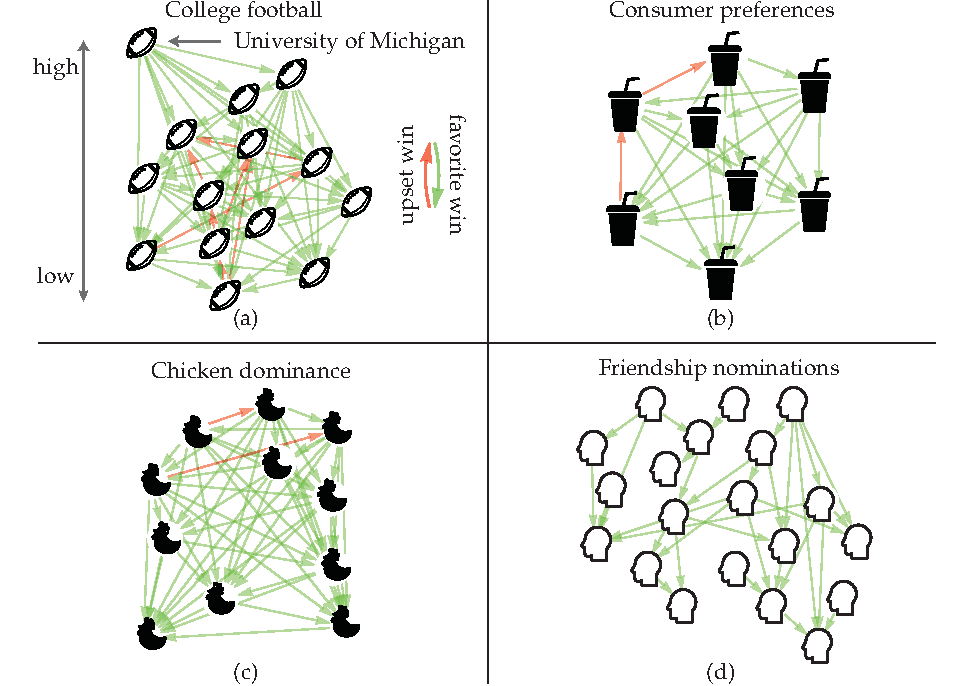
\includegraphics{max_dissertation//chapters//figures//chp1/hierarchy-examples.pdf}
    \caption{Four examples of hierarchy structure in networks. (a) American football matches played in the 2022 Big Ten conference football season~\cite{Football22}.  The hierarchical structure is represented vertically, with better teams located higher. Arrows run from the winner to the loser of a match, colored green if the higher ranked team wins, red if the lower ranked team wins. (b) Consumer preferences between pairs of sodas~\cite{DAK00}. (c) Observed dominance interactions (pecks) among 11 chickens~\cite{MA34}. (d) Unreciprocated friendship nominations among 20 high school students~\cite{AddHealth}.}
    \label{fig:hierarchy-examples}
\end{figure}

Figure~\ref{fig:hierarchy-examples}a contains football matches played within the 2022 Big Ten football conference~\cite{Football22}. Each arrow points from the winner to the loser of a match, information that was suppressed in the undirected Figure~\ref{fig:community-examples}a. The University of Michigan was undefeated in this (carefully chosen) season as indicated by all arrows pointing away from its node and by its position at the top of the football hierarchy. In this case placement on the hierarchy is meant to reflect strength in the game of football, and we would expect that better teams win more often than lower ranked ones. Particularly we may assume that the outcome of any given match is driven by the difference in skill between the participating teams. Although the teams and fans are generally aware of these relative strengths, there is not a "true" hierarchy to refer to like the conference group structure. The positions in the hierarchy must instead be deduced from the observed matches. 

There are many ways to determine a hierarchy from the match outcomes. Collegiate football formalizes this inference through an annual poll of team coaches to determine the highest ranked teams who may then advance to the post-season playoff bracket. In Figure~\ref{fig:hierarchy-examples}a, the vertical hierarchy is instead arranged in order to maximize the number of times the higher ranked team wins (the 57 green arrows) and minimize the upset victories (the 7 red arrows). The other networks of Figure~\ref{fig:hierarchy-examples} are likewise arranged to minimize such \emph{violations} of their hierarchies. We discuss other methods for arriving at such a ranking in Section~\ref{sec:BT-model}. 

The presence of upsets means that the data does not fully respect the hierarchy. One might hope that there is some other ordering of the teams that is fully coherent, lacking any such upsets, but the intransitivity of the results prevents this. In the football example Minnesota beat Nebraska, Nebraska beat Iowa, and Iowa beat Minnesota in a rock-paper-scissors arrangement. One of these three matches would therefore be recorded as an "upset" under any ordering of the teams. In fact any ordering of this season will have at least 7 upsets as in the ordering plotted in the figure. This tension between the hierarchy and the realized results is analogous to how not all edges lie within the groups of Figure~\ref{fig:community-examples}. The degree to which the outcomes conform to a hierarchy gives insight to its strictness. 

Many of the models used to describe hierarchies were initially developed and are often used in the world of sports, yet similar concepts can be applied to understand status and quality in other contexts. Figure~\ref{fig:hierarchy-examples}b shows a hierarchy of 8 different flavored sodas. In this network wins indicate if most assessors surveyed by Duineveld~\etal~prefer one soda over another in a \emph{paired comparison} study~\cite{DAK00}. Again no total ordering of the sodas is possible as the revealed preferences are not strictly transitive, although there are certain sodas that generally fare better in these comparisons. Such surveys and inferences are often used to make sense of A/B testing of various types of products and establish the aggregate consensus of quality and preferences. These methods are similarly used in reinforcement learning to assess and tune large language model outputs based upon human preferences~\cite{CLBMLA17}.

Turning to animals, the social hierarchy of a flock of 11 Brown Leghorn chickens is plotted in Figure~\ref{fig:hierarchy-examples}c~\cite{MA34}. Here the arrows represent when one chicken pecks another but is not pecked in return, taken as a sign of dominance. The chickens organize into a pecking order where the higher chicken tends to peck the lower chicken on the ladder. This animal behavior research is in fact the source of the phrase "pecking order" colloquially used to refer to all sorts of hierarchies. In this flock of 11, the chicken at the bottom of the pecking order is pecked by all above it while there is more competition and ambiguity at the top. 

Figure~\ref{fig:hierarchy-examples}d shows a similar social hierarchy, now of surveyed friendship nominations among 20 students of a small U.S. high school~\cite{AddHealth}. Although we may think of friendship as a two-way street, this reciprocity is not always borne out in survey data. Often student A names student B as their friend but student B does not name student A back. We can interpret this as a "win" for student B in the social hierarchy, and that they are likely of higher social status than student A. In the school of this figure a clear hierarchy emerges where higher status students consistently dominate the lower ranked students in this manner. 

Each of the directed network representations in Figure~\ref{fig:community-examples} foregoes further context unique to each setting. The football match network, for example, neglects idiosyncratic details like player injuries or home-field advantages that can influence the outcome of any given match. Such events, however, do not have a clear analog within, say, the pecking order of chickens. By reducing the systems down to a directed pattern of "wins" and "losses," we can directly compare them to each other. In Chapter~\ref{chp:hierarchies} of this thesis we discuss how this framework enables us to observe how the nature and strength of these hierarchies differ across settings.